\documentclass[11pt,a4paper]{article}
\usepackage[margin=27mm]{geometry}
\usepackage{fontspec,booktabs,array,hyperref,graphicx}
\setmainfont{STIXGeneral}
\setlength{\parindent}{0pt}\setlength{\parskip}{5pt}
\begin{document}
\begin{center}{\Large Complete manuscript comparison}\\[3pt]
Overview v18: transitive string markings\end{center}
This edition covers 19 topics and 52 measured originals. The 106 accessible originals comprise 52 measured mathematical originals, 53 awaiting mathematical recovery and measurement, and one editorial, L022. The 55 unavailable originals remain archived. L022 contains no principal mathematical result to recover: it stays accessible, with no factor or measured credit.

L047 joins B. All 18 other whole-topic records and all 51 earlier individual records retain their exact v17 values. B's whole factor changes from $1.094035$ to $0.971866$: the enlarged replacement is a written expansion. The new L047 conditional is $3.629111$, after acquisition of both whole common papers and all required topic premises. The complete written factor for each topic is $\sum_i c(S_i)/(c(U)+\sum_i c(A_i))$: full common theory and all complete applications are paid once within that topic.

Each topic retains its adopted nonwhitespace-character coordinate. There is no pooled factor or cross-topic deduction, and no inferred minimum proof length. Executable software is excluded on both sides; mathematical proof and algorithm prose remain counted.
\begin{center}\small\begin{tabular}{lrrrrr}\toprule
Topic & Originals & Sources & Common & Applications & Factor\\\midrule
A & 9 & 273,937 & 66,140 & 136,125 & 1.354 \\
B & 6 & 144,877 & 74,303 & 74,768 & 0.972 \\
C & 5 & 118,433 & 30,437 & 61,248 & 1.292 \\
D & 3 & 47,894 & 15,632 & 29,855 & 1.053 \\
E & 5 & 140,286 & 57,473 & 32,337 & 1.562 \\
F & 2 & 69,825 & 15,876 & 27,398 & 1.614 \\
G & 2 & 73,199 & 30,928 & 85,207 & 0.630 \\
Representation & 2 & 60,472 & 36,715 & 45,437 & 0.736 \\
Chamber & 2 & 34,177 & 15,199 & 21,254 & 0.938 \\
Matching & 1 & 37,951 & 16,732 & 17,168 & 1.119 \\
ChiralEnumeration & 1 & 27,594 & 8,831 & 23,171 & 0.862 \\
Operations & 3 & 200,630 & 58,215 & 100,379 & 1.265 \\
Gluing & 1 & 27,081 & 28,416 & 11,565 & 0.677 \\
RankContraction & 1 & 15,530 & 6,937 & 10,555 & 0.888 \\
LocallyProjective & 2 & 26,490 & 25,498 & 11,966 & 0.707 \\
MathieuCensus & 1 & 13,736 & 5,516 & 35,862 & 0.332 \\
RankAugmentation & 1 & 33,604 & 13,904 & 14,096 & 1.200 \\
Mixes & 3 & 156,570 & 34,757 & 68,693 & 1.513 \\
LCD & 2 & 58,756 & 32,300 & 66,886 & 0.592 \\
\bottomrule\end{tabular}\end{center}
The \href{topics.csv}{19-topic CSV} and \href{applications.csv}{52-original CSV} preserve exact fractions and complete component costs. Factors below one mean written expansion and remain visible. The separate source admissions define the corrected principal contracts; this overview creates no additional proof, question or formalization credit.
\newpage
\section*{Individual comparisons: first 26 originals}
The conditional factor is $c(S_i)/c(A_i)$ after acquiring the \emph{whole} common theory and all actual required mathematical, computational and data premises. Every complete local application or companion bundle remains charged.
\begin{center}\small\begin{tabular}{llrrr}\toprule
Original & Topic & Source & Application & Factor\\\midrule
L032 & A & 16,558 & 8,228 & 2.012 \\
L034 & A & 21,433 & 5,801 & 3.695 \\
F016 & A & 43,983 & 15,436 & 2.849 \\
F013 & A & 25,562 & 6,241 & 4.096 \\
L035 & A & 51,019 & 14,514 & 3.515 \\
N009 & A & 36,824 & 28,130 & 1.309 \\
L128 & A & 18,424 & 8,825 & 2.088 \\
L012 & A & 32,767 & 23,401 & 1.400 \\
L121 & A & 27,367 & 25,549 & 1.071 \\
N001 & B & 14,519 & 7,371 & 1.970 \\
N003 & B & 17,780 & 9,155 & 1.942 \\
N008 & B & 18,009 & 11,132 & 1.618 \\
L030 & B & 22,704 & 12,286 & 1.848 \\
L040 & B & 51,894 & 29,321 & 1.770 \\
L047 & B & 19,971 & 5,503 & 3.629 \\
L088 & C & 13,166 & 11,311 & 1.164 \\
N013 & C & 27,361 & 15,815 & 1.730 \\
L108 & C & 12,849 & 10,075 & 1.275 \\
F014 & C & 20,577 & 6,962 & 2.956 \\
L068 & C & 44,480 & 17,085 & 2.603 \\
L066 & D & 20,916 & 10,989 & 1.903 \\
L074 & D & 20,661 & 13,367 & 1.546 \\
L104 & D & 6,317 & 5,499 & 1.149 \\
L079 & E & 21,212 & 1,858 & 11.417 \\
L083 & E & 20,904 & 2,922 & 7.154 \\
L021 & E & 29,594 & 14,452 & 2.048 \\\bottomrule\end{tabular}\end{center}
B pays the entire old 16-page common paper and the whole 10-page addition, plus all six applications (30 pages):
\[R_B=\frac{144,877}{44,905+29,398+74,768}=0.971866.\]
The replacement is 4,194 characters longer overall. The common addition costs 29,398 characters, separately visible as a new acquisition stage in B's reader. L047 contributes its full twelve-page source and three-page application: $19,971/5,503=3.629111$ conditionally. The five earlier conditional records are unchanged in all thirty coordinates.
\newpage
\section*{Individual comparisons: remaining 26 originals}
\begin{center}\small\begin{tabular}{llrrr}\toprule
Original & Topic & Source & Application & Factor\\\midrule
L056 & E & 15,871 & 4,144 & 3.830 \\
L043 & E & 52,705 & 8,961 & 5.882 \\
L014 & F & 25,574 & 11,504 & 2.223 \\
L007 & F & 44,251 & 15,894 & 2.784 \\
L009 & G & 49,891 & 23,544 & 2.119 \\
L092 & G & 23,308 & 61,663 & 0.378 \\
F010 & Representation & 25,348 & 10,985 & 2.308 \\
L126 & Representation & 35,124 & 34,452 & 1.020 \\
L008 & Chamber & 20,159 & 7,571 & 2.663 \\
N016 & Chamber & 14,018 & 13,683 & 1.024 \\
F015 & Matching & 37,951 & 17,168 & 2.211 \\
L028 & ChiralEnumeration & 27,594 & 23,171 & 1.191 \\
N005 & Operations & 122,002 & 49,595 & 2.460 \\
N006 & Operations & 55,740 & 38,479 & 1.449 \\
N007 & Operations & 22,888 & 12,305 & 1.860 \\
L010 & Gluing & 27,081 & 11,565 & 2.342 \\
L037 & RankContraction & 15,530 & 10,555 & 1.471 \\
L084 & LocallyProjective & 2,071 & 4,857 & 0.426 \\
L095 & LocallyProjective & 24,419 & 7,109 & 3.435 \\
L073 & MathieuCensus & 13,736 & 35,862 & 0.383 \\
L020 & RankAugmentation & 33,604 & 14,096 & 2.384 \\
F005 & Mixes & 57,753 & 31,077 & 1.858 \\
L016 & Mixes & 35,506 & 15,125 & 2.348 \\
F007 & Mixes & 63,311 & 22,491 & 2.815 \\
L050 & LCD & 24,674 & 37,432 & 0.659 \\
F017 & LCD & 34,082 & 29,454 & 1.157 \\\bottomrule\end{tabular}\end{center}
B's separate inventory contains 17 whole distinct files: eight required or auxiliary programs, two optional validations, five operational drivers and two partial Lean files. The required files occupy 24,859 original bytes. The roster file \texttt{run.g} remains a required premise. Both complete seven-page code appendices and all ten raw programs are disclosed as alternatives; they are not added together or used for a software-inclusive factor.

L047's corrected principal contract retains 23 finer ancillary Table 3 reports as attributed statements, not regenerated results. The source's conjecture was already resolved in L044; this comparison credits no new answer. N001 remains a complete authored rendering, with its original PDF unknown. The source side otherwise retains five whole PDFs, including L040's identification cover. Fourteen inherited Lean declarations remain partial evidence.

All software-inclusive and pooled factors remain null. Historical software, external proofs, complete graphics and full formalization costs are unknown. Operations retains its text-only sensitivity; E retains the source's Magma/$L_2$-quotient attribution and all source qualifications. Prior overviews remain historical records.
\newpage
\section*{Whole topics}
Grey bars show the complete originals in each row's adopted coordinate. Replacement bars stack the entire common theory and all applications. The axis starts at zero; the table gives the factors.
\begin{center}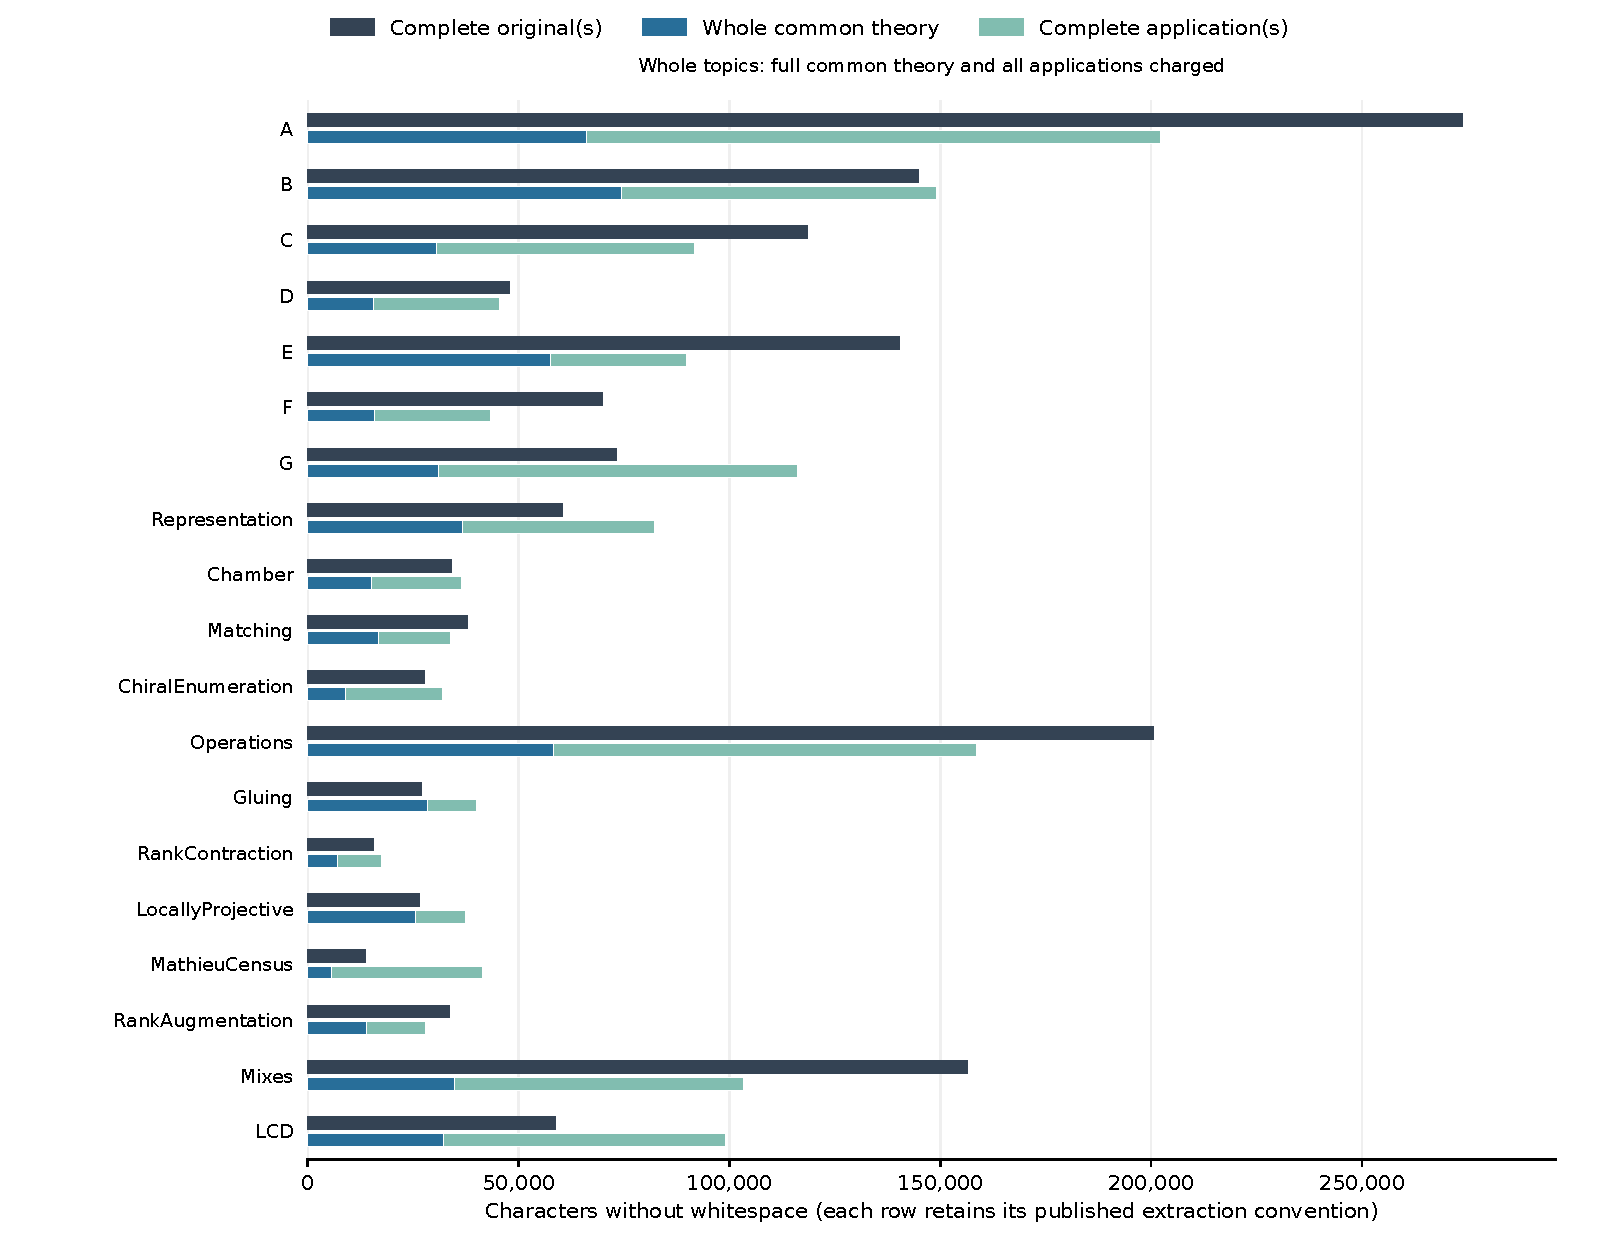
\includegraphics[width=\linewidth]{whole_topics.pdf}\end{center}
The 57 bars cover all 19 topics. Necessary finite certificates and retained external premises do not become optional because their software or external proof costs are outside this manuscript comparison.
\newpage
\section*{Conditional lengths: first 26 originals}
Whole common theory and required premises are acquired in advance. Grey and teal bars compare complete source and local application text; the whole-topic table still pays the common theory.
\begin{center}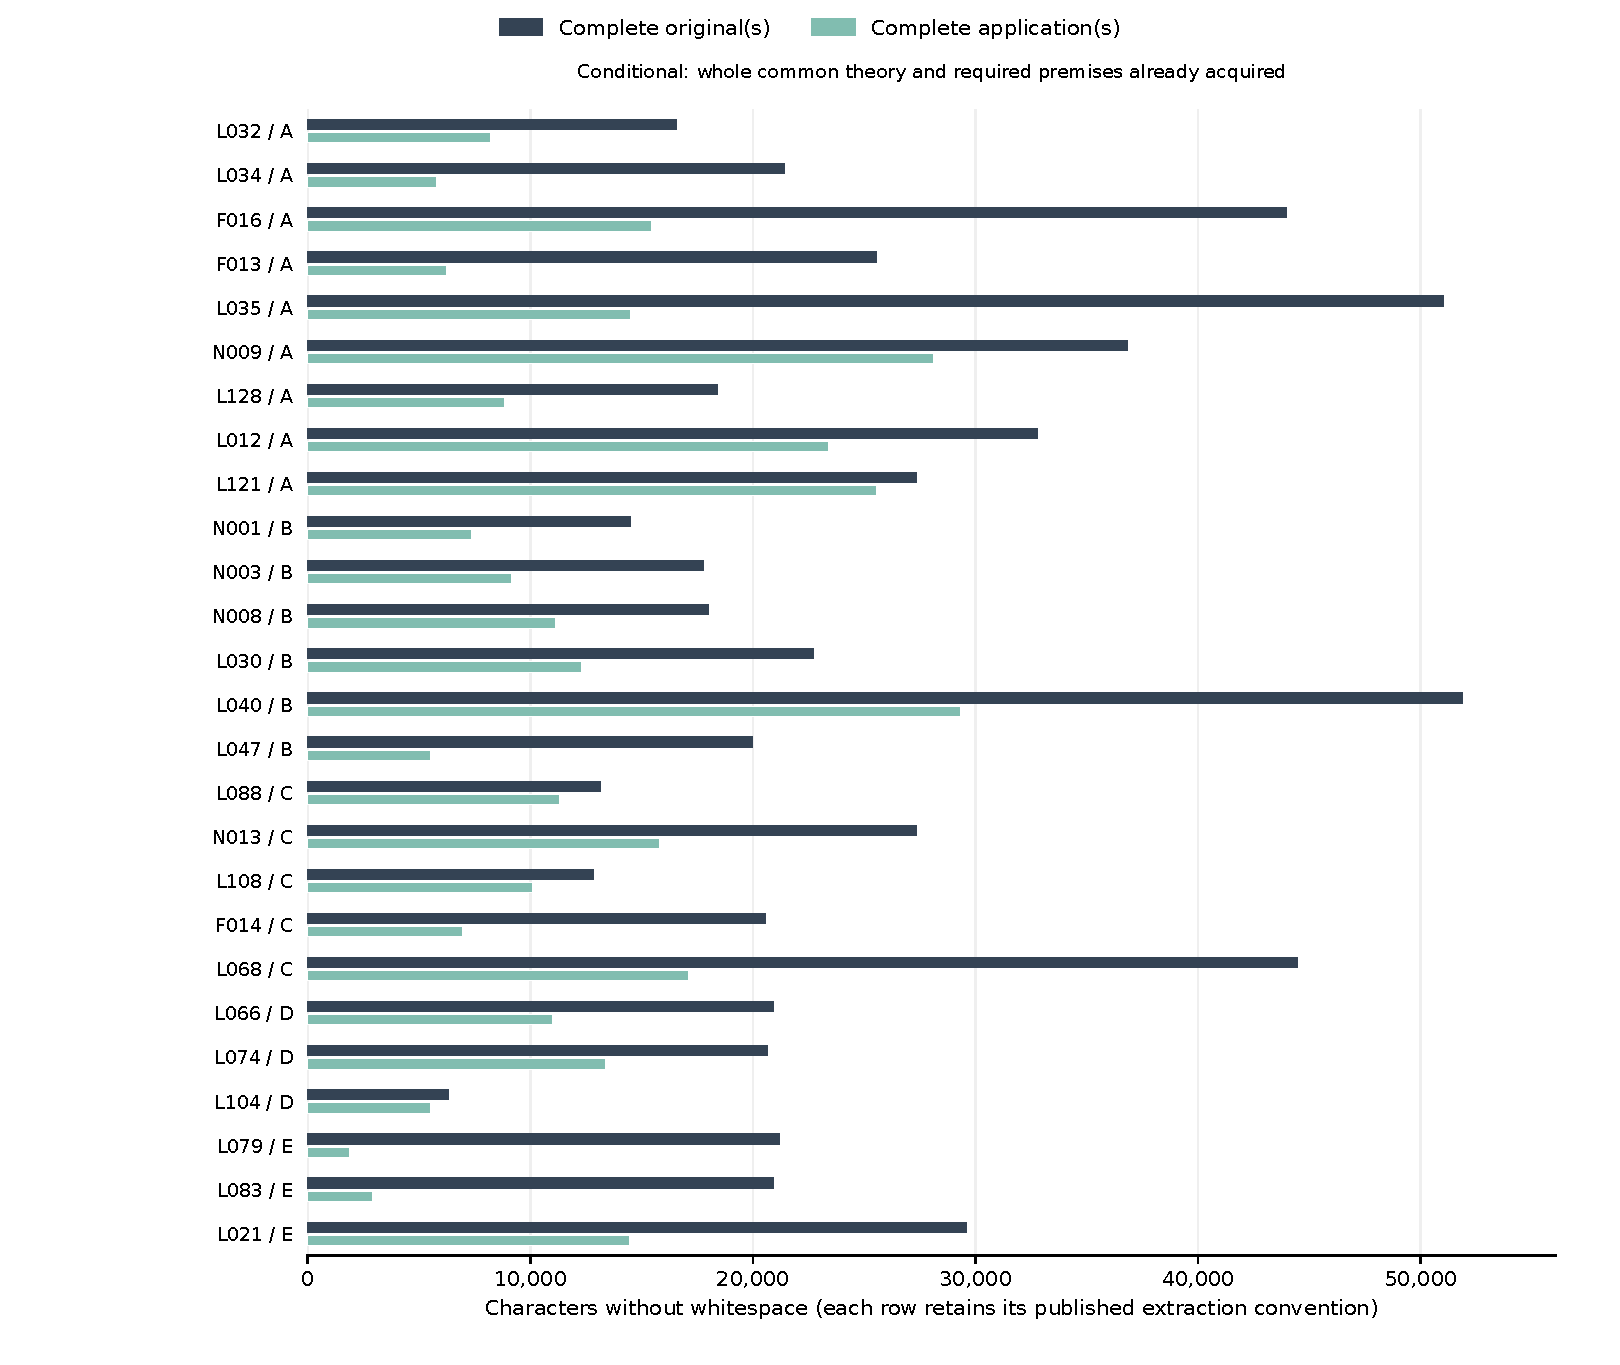
\includegraphics[width=\linewidth]{conditional_1.pdf}\end{center}
\newpage
\section*{Conditional lengths: remaining 26 originals}
All complete companion papers remain charged. Source order is documentary, not an optimal acquisition order or a claimed sawtooth.
\begin{center}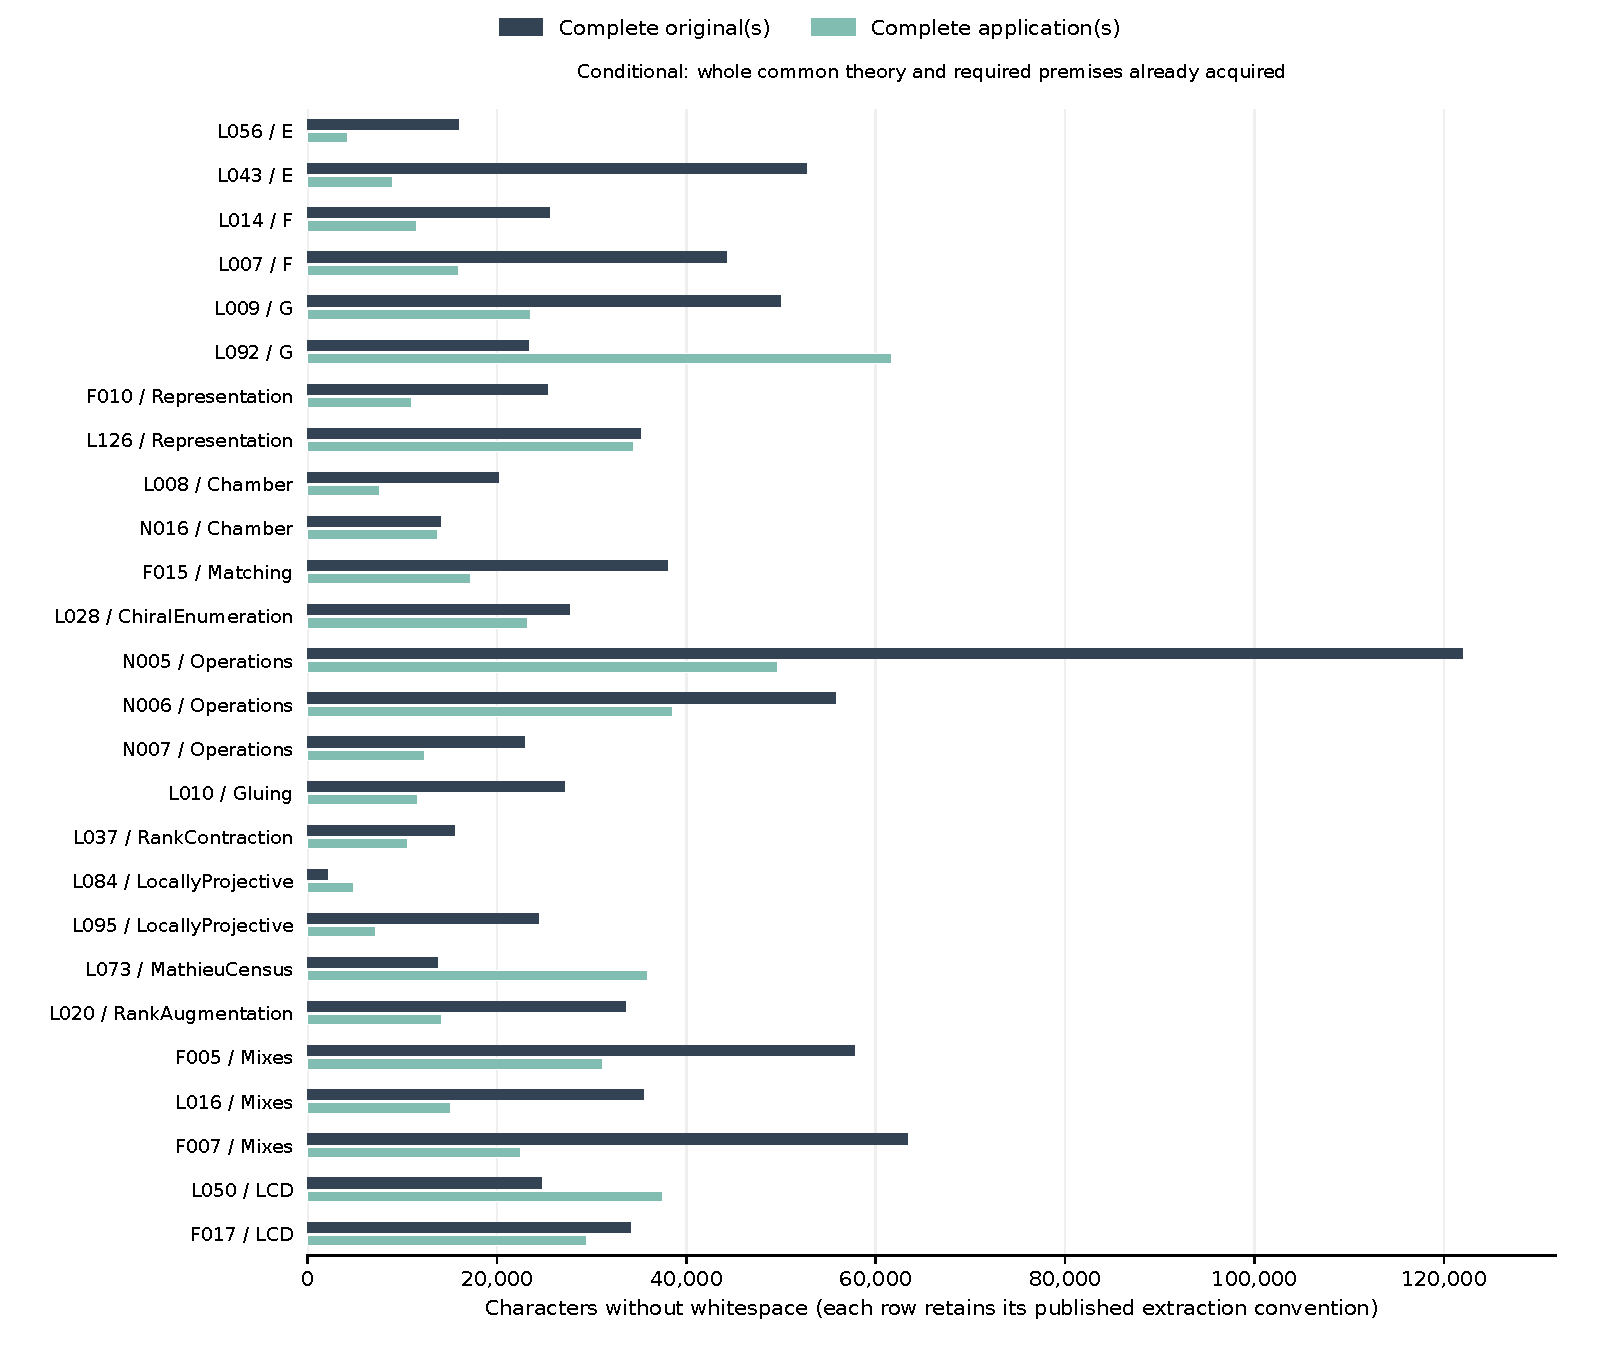
\includegraphics[width=\linewidth]{conditional_2.pdf}\end{center}
This edition supplies 71 exact manuscript comparisons and 161 plotted bars. The B6 numerical author is enumeration\_volume; root distinctly reviewed and adopted those calculations and their inputs. The new L047 science is by enumeration\_review and the input author is rewrite\_termination. Earlier B authorship and the bounded finite-neighbor review roles remain disclosed in the topic packet. This overview reuses accepted costs. L022 has no mathematical recovery credit or numerical bar; no new conjecture or priority claim is made.
\end{document}
